\documentclass[preprint, sort&compress]{elsarticle}
\usepackage{amsmath}
\usepackage{amssymb}
\usepackage{amsthm}
\usepackage{amsfonts}
\usepackage{amsbsy}
\usepackage{amstext}
\usepackage{amsmath}
\usepackage{amsfonts}
\usepackage{amssymb}
\usepackage{amsthm}
\usepackage{amstext}
\usepackage{mathrsfs}
\usepackage{graphpap}
\usepackage[utf8]{inputenc}
\usepackage{graphicx}
\usepackage{subcaption}
\usepackage{graphics,graphicx}
\usepackage{multicol}
\usepackage{booktabs}
\usepackage{array}
\usepackage{siunitx}
\usepackage{abstract}
\usepackage{hyperref}
\usepackage{siunitx}
\hypersetup{colorlinks = true, allcolors = blue}
\usepackage[nameinlink,noabbrev]{cleveref}
\renewcommand{\abstractname}{}
\renewcommand{\absnamepos}{empty}
\newcommand{\R}{\mathbb{R}}
\newcommand{\e}{\varepsilon}
\newcommand{\f}{\mathfrak{F}}
\newcommand{\Q}{\mathbb{Q}}
\newcommand{\N}{\mathbb{N}}
\newtheorem{teor}{Theorem}
\newtheorem{lemma}{Lemma}
\makeatletter \def
\ps@pprintTitle{
     \let\@oddhead\@empty \let\@evenhead\@empty
    \let\@oddfoot\@empty
    \let\@evenfoot\@oddfoot
}
\makeatother
\makeatletter
\def\ps@pprintTitle{
    \let\@oddhead\@empty
    \let\@evenhead\@empty
    \let\@oddfoot\@empty
    \let\@evenfoot\@oddfoot
}
\makeatother
\begin{document}
    \begin{frontmatter}
        \title{
            Optimal vaccination preventive policies for COVID-19\\
            \large{Research Report (WHO-SAGE)}
        }
        \author{Grupo ITSON-CONACyT-UNISON\\
            September 18, 2020
        }

\end{frontmatter}

	\section{Introduction}
		In late December 2019, a new virus's appearance is reported in Wuhan City, Hubei Province, China. Called SARS-CoV2, it is the virus that causes the 2019 coronavirus disease (COVID-19) and that, very quickly since its appearance, has spread throughout much of the world, causing severe problems for health systems of all the countries in which it is present \cite{Who12020}. On March 11, 2020, the World Health Organization declared the epidemic by COVID-19 as a pandemic.  Around 118,000 cases at that time, distributed in 114 countries and with around 4,291 deaths \cite{Who512020}. In Latin America, the first
detected case of COVID-19 occurred in Brazil on February 26, and in Mexico, the first case was reported on February 27, quickly spreading throughout the country \cite{Ajrm2020,Acuna2020}.

Various control measures have been implemented in all the countries where the disease is present, with quarantine, isolation, and social distancing being the main ones. Despite the measures that different governments have taken to mitigate the epidemic, it has not been controlled. The number of cases and deaths from the disease continues to increase in many countries of the world. On the other hand, since the new coronavirus's appearance, the international scientific community has been working to understand the nature of the virus. They mainly focus on the spreading mechanisms between individuals, developing vaccines and treatments to reduce the number of infections and fatality cases. To get a clearer understanding of different vaccination strategies and their consequences on the number of infected individuals, mathematical models have taken a leading role. The use of various mathematical tools such as SIR and SEIR models has helped to describe epidemics properties around the globe.

Initially, these models have been used to estimate the basic reproductive number associated with the disease and estimate different parameters involved in its spread, such as contagion rates, incubation periods, and recovery rates. They are also being used to propose and evaluate the effect of various control measures, such as quarantine \cite{Acuna2020,Wang2020,Marimuthu2020,Liu2020,Ghosh2020,Calvetti2020,Shaikh2020}.

On the other hand, a widely used tool to propose optimal scenarios for applying vaccines or treatments is the optimal control theory. With this tool, it is possible to find scenarios in which the application of the vaccine minimizes the damage caused by the disease and the cost of its application. Some results about it have been applied to control other diseases for humans and animals \cite{Asano2008,Rodrigues2014,Tchuenche2011,Malik2016,Jaberi2014}.

In this work, we present a mathematical model to describe the propagation disease and vaccination dynamics of COVID-19. An analysis of the basic reproductive number is shown, providing conditions, in terms of the vaccination parameters, that allow both reducing the value of $\mathcal{R}_{0}$ and lowering its value below one. Finally, optimal scenarios for applying a preventive vaccine are also presented through optimal control theory. It is important to stress that we used the Mexican Ministry of Health data to estimate the proposed model's parameters before the vaccine application. In this way, we have the possibility of analyzing the effect of the vaccine, maintaining a base of values for the model parameters, and thus being able to manipulate only the parameters corresponding to vaccination. 
 	\section{Mathematical model formulation}\noindent In this section, we formulate our baseline mathematical model, which additionally to the transmission dynamics, includes vaccination. In order to build our model, we follow the classical Kermack-McKendrick approach. Our model splits the population in seven different classes: Susceptible $(S)$, exposed $(E)$, symptomatic infected $(I_S)$, asymptomatic infected $(I_A)$, recovered $(R)$, death $(D)$ and vaccinated $(V)$ individuals. It is important to mention that $I_{S}$ represents the proportion of symptomatic individuals who will later report to some health medical center. Additionally to the classical process an individual might follows during infection, in our model, we assume that reinfection is possible after a period of time. We model the vaccination process considering some assumptions: i) Vaccination is applied to all the alive individuals except those in the symptomatic class. In this situation, vaccines are distributed over individuals on the $S$, $E$, $I_A$, and $R$ classes. ii) The vaccine has preventive nature, that is, only reflected in the susceptible individuals $(S)$. iii) People will only get one vaccine during the campaign. iv) Vaccines do not necessarily have a hundred percent of effectivity, which implies that some vaccinated people can get the disease. We denote the effectivity rate by $\epsilon$. Based on these assumptions our model becomes

\begin{equation}\label{model1}
  \begin{aligned}
	S'(t)&=\mu \bar{N}-\frac{\beta_S I_S+\beta_AI_A}{\bar{N}}S-(\mu+\lambda_V)S +\delta_V V+ \delta_R R\\
	E'(t)&= \frac{\beta_S I_S+\beta_AI_A}{\bar{N}}S+(1-\epsilon) \frac{\beta_S I_S+\beta_AI_A}{\bar{N}}V-(\mu+\delta_E) E \\
	I'_S(t)&= p \delta_E E-(\mu+\alpha_S) I_S\\
	I'_A(t)&= (1-p) \delta_E E-(\mu+\alpha_A) I_A \\
	R'(t)&= (1-\theta) \alpha_S I_S+\alpha_A I_A-(\mu+\delta_R) R \\
	D'(t)&= \theta \alpha_S I_S \\
	V'(t)&= \lambda_V S-(1-\epsilon)  \frac{\beta_S I_S+\beta_AI_A}{\bar{N}}V-(\mu+\delta_V) V
      \end{aligned}
\end{equation}
where $\bar{N}(t)=S(t)+E(t)+I_S(t)+I_A(t)+R(t)+V(t)$ and $N=\bar{N}+D$. Parameters description of system~\ref{model1} is given in Table \ref{table1}.
\begin{table}[h!]
    \begin{tabular}{>{\centering}p{0.2\textwidth}p{0.6\textwidth}}
			\toprule
			Parameter & Description
      \\
      \midrule
			$\mu$ &  Death rate
			\\
            $\beta_S$ & Infection rate between susceptible and symptomatic infected
			\\
            $\beta_A$ & Infection rate between susceptible and asymptomatic infected
			\\
            $\lambda_V$ & Vaccination rate
			\\
            $\delta_{V}^{-1}$ & Immunity average time by vaccination
			\\
            $\epsilon$ &  Effectivity rate of the vaccination
			\\
            $\delta_{E}^{-1}$ & Average time of the incubation period \\
			$p$ & Proportion of symptomatic individuals  \\			
            $\alpha_{S}^{-1}$ &  Average output time of symptomatic individuals due to death or recovery  \\
            $\theta$ & Proportion of symptomatic individuals who die due to the disease \\ 
			$\alpha_{A}^{-1}$ & Recovery average time of asymptomatic individuals  \\ 					 
            $\delta_{R}^{-1}$ &  Immunity average time by disease \\
      \bottomrule
		\end{tabular}
  \caption{Parameters definition of system~\ref{model1}.}\label{table1}
\end{table}
 	\section{Parameter fitting}\noindent Mathematical models for COVID-19 have shown that the parameters values are not necessarily the same in each country. For this reason, we use data from Mexico city plus the surrounding metropolitan area to estimate some parameter values of system~\ref{model1}. These values will be used to exemplify our results. For the parameter estimation process, we fixed some parameter values according the literature, and then followed a two-stages process: i) before, and ii) after mitigation measures were implemented. In both stages, we used model~\ref{model1}, with no vaccination ($\lambda_V$ and $V = 0$). For the first stage, we consider the dates from the first day of symptoms onset reported (February 19) until March 23, 2020. For the second stage, we took a month later than mitigation measures were implemented, that is, from March 23 to April 23, 2020, and results are shown in Figure~\ref{Figure1}. It is important to stress that the second stage is used to partially represent the non-pharmaceutical interventions, which implies a reduction of contact transmission rates. Parameter values are summarized in Table~\ref{table_icparam}, while fixed parameters values are shown in Table~\ref{table_fixparam}.

















\begin{table}[h!]
\begin{center}
    \begin{tabular}{>{\centering}p{0.2\textwidth}p{0.4\textwidth}p{0.2\textwidth}}
        \toprule
        Parameter & 95\% Confidence Interval & Quantile 50
        \\
        \midrule
        $\beta_S$ & $[\num{0.6689}, \num{1.191}]$   &  $\num{0.9303}$
        \\
        $\beta_A$ & $[\num{0.5019}, \num{0.7867}]$  &  $\num{0.6441}$
        \\
        $p$       & $[\num{0.06088}, \num{0.2239}]$ &  $\num{0.1213}$
        \\
        $\xi$     & $[\num{0.3707}, \num{0.4113}]$  & $\num{0.3905}$
        \\
\\
    \bottomrule
\end{tabular}
  \caption{Estimated values for some parameters of system~\ref{model1}.}\label{table_icparam}
\end{center}
\end{table}

\begin{table}[h!]
    \begin{center}
        \begin{tabular}{>{\centering}p{0.2\textwidth}p{0.2\textwidth}p{0.2\textwidth}}
            \toprule
            Parameter & Value & References
            \\
            \midrule
            $\delta_{E}^{-1}$ & \SI{5.1}{days}   &  \cite{Tian2020}
            \\
            $\alpha_{S}^{1}$  & \SI{5.97}{days}  &  \cite{Acuna2020}
            \\
            $\alpha_{A}^{-1}$ & \SI{10.81}{days} & \cite{Acuna2020}
            \\
            $\delta_{R}^{-1}$ & \SI{1}{years}     &
            \\
            $\mu^{-1}$        & \SI{75}{years}   &
            \\
            \bottomrule
        \end{tabular}
        \caption{
            Fixed parameters values of system~\ref{model1}.
        }
        \label{table_fixparam}
    \end{center}
\end{table}


Figure~\ref{Figure1} shows the fitting curves for the two time periods. With
the obtained parameters, we simulated the evolution of the number of infected
individuals starting on February 19, 2020 until July 2022. With  these dates,
it is possible to observe two outbreaks (Figure~\ref{Figure2}), where the
second one is referred to as the second wave of COVID-19. With this scenario,
it is possible to evaluate the effect of different vaccination strategies,
which we consider to start to be applied on March 2021, which is the time prior
to the onset of the second wave.
\begin{figure}[!h]
  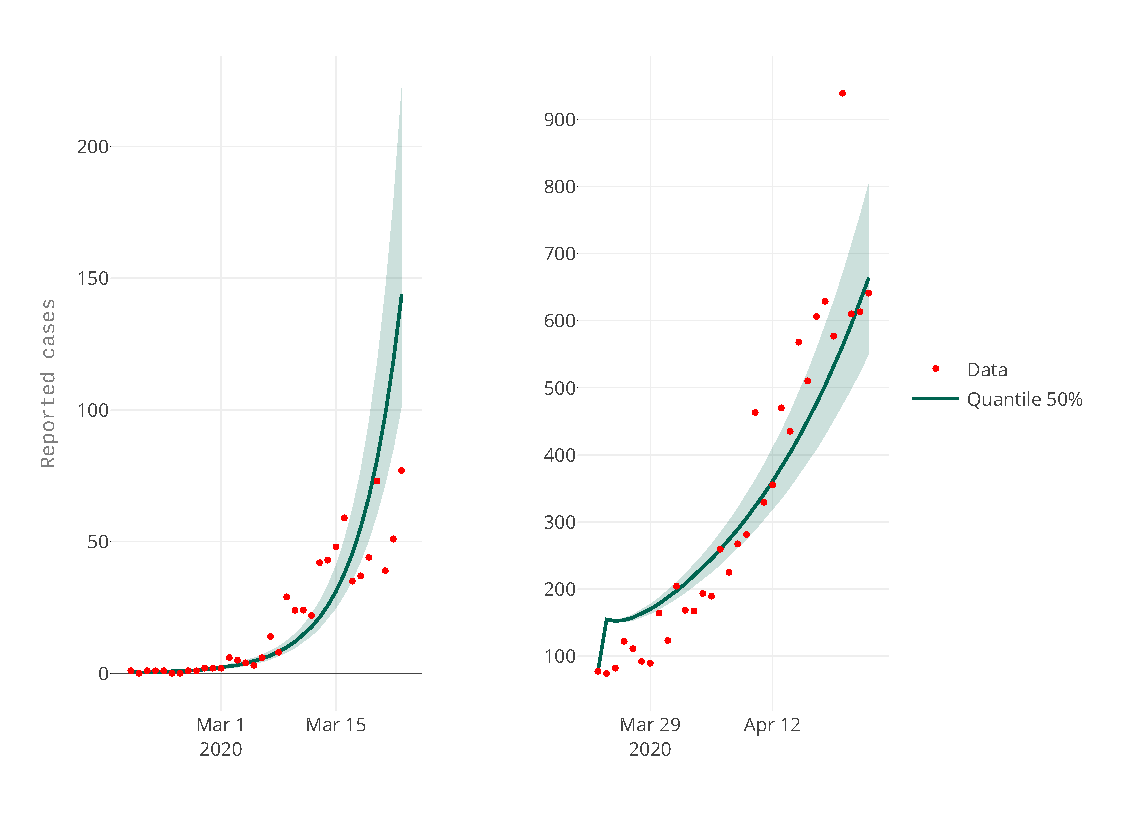
\includegraphics[width=\textwidth]{FittingCurves.eps}
  \caption{Fitting curves for the early phase of the COVID-19 outbreak in
      Mexico City plus the surrounding metropolitan area. The left side shows
      the outbreak from February 19 to March 23, 2020. The right side shows the
      outbreak from March 23 to April 23, 2020.}
  \label{Figure1}
\end{figure}
\pagebreak
\begin{figure}[!h]
  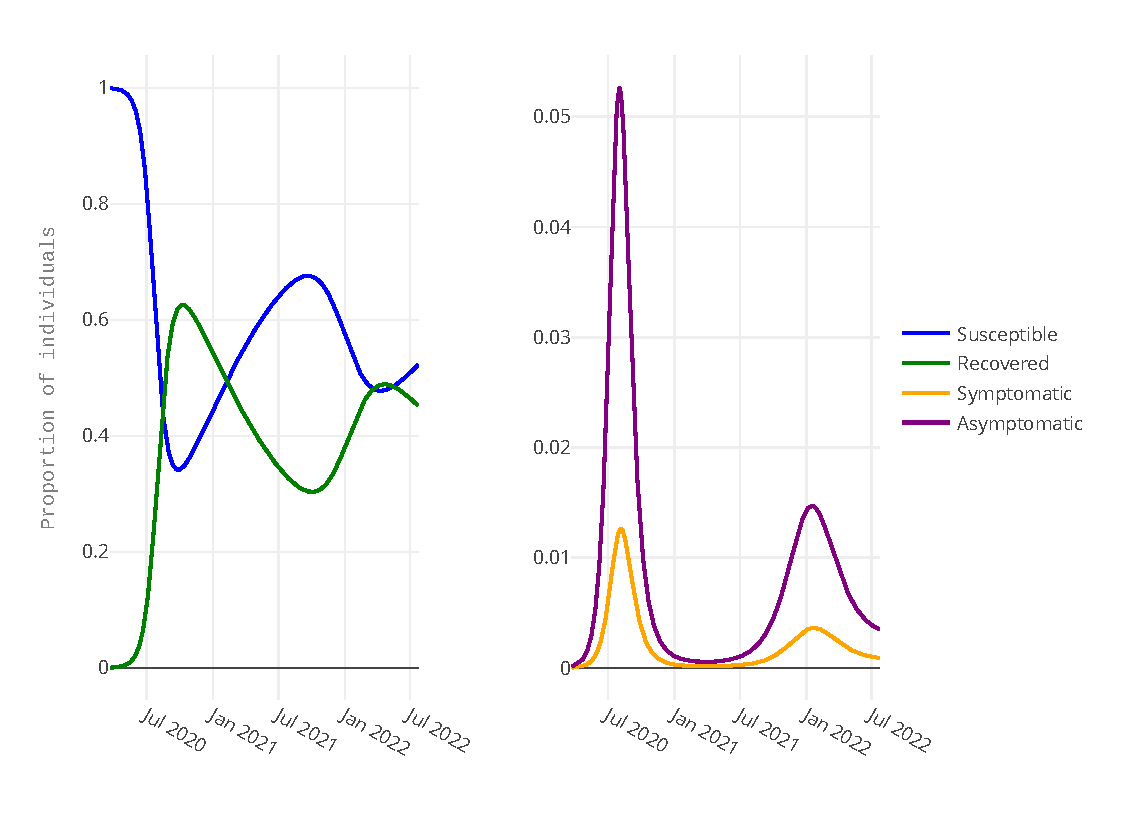
\includegraphics[width=\textwidth]{Solutions.eps}
  \caption{Dynamics populations without vaccination process. Here,
      system~\ref{model1} is reduced when considering $\lambda_V = \delta_V =
      0$, $\epsilon = 1$, and $V(0) = 0$.}
    \label{Figure2}
\end{figure}
\pagebreak 	\section{Vaccination Model Analysis}
In this section, we use the estimated parameters from the previous section to analyze Model (\ref{model1}) and the effect of the vaccine. Some plausible scenarios are presented, depending on the effectiveness of the vaccine,  as well as the rate of vaccination.

In the first instance, it has been shown that the interest region of the state variables of the system is positively invariant. This implies that any solution with initial conditions within that region will remain within it.







Now, using the next-generation matrix method  \cite{Diekmann1990, Van2002}, the basic reproductive number for system (\ref{model1}) is given by









\begin{equation}\label{Rv}
R_{V}=R_S+R_A
\end{equation}
with

\begin{eqnarray*}
R_S&=&\frac{p\beta_S\delta_E(\mu+\delta_V+(1-\epsilon) \lambda_V)}{(\mu+\delta_E)(\mu+\delta_V+\lambda_V)(\mu+\alpha_S+\mu_S+\lambda_T)}\\ 
 R_A&=&\frac{(1-p)\beta_A\delta_E(\mu+\delta_V+(1-\epsilon) \lambda_V)}{(\mu+\delta_E)(\mu+\delta_V+\lambda_V)(\mu+\alpha_A+\mu_A)}.\nonumber
\end{eqnarray*}
 Note that each sum of $ R_ {V} $ represents the contribution of the symptomatic and asymptomatic infected, respectively, to the spread of the disease.

Now, following the ideas of Alexander et.al. \cite{Alexander2004}, expression for $R_V$ can be rewritten as

\begin{equation}\label{Rv2}
R_{V}=R_0\left(1- \frac{\epsilon \lambda_V}{(\mu+\delta_V+\lambda_V)}\right)
\end{equation}
where $R_0$ is the basic reproduction number of system without vaccine. Note that $\left(1- \frac{\epsilon \lambda_V}{(\mu+\delta_V+\lambda_V)}\right)<1$, Therefore, this factor which saves the parameters corresponding to the application of the vaccine will allow us to modulate the value of $ R_0 $. In the first instance, if $ R_0 <1 $, then $ R_V <1 $. But, if $ R_0> 1 $, we wonder if the application of the vaccine can lower $R_V$ value below 1. In this sense, it is easy to prove that, if

\begin{equation}\label{condition1}
\epsilon>\frac{(R_0-1)(\mu+\delta_V+\lambda_V)}{R_0\lambda_V},
\end{equation}

\noindent it is possible to reduce the value of $ R_V $ below one, of course with the necessary conditions in terms of vaccination. That is, there is a region in the parameter space in which it is possible to reduce the value of $ R_V $ below one, considering adequate efficacy, vaccination rate and duration of the effect of the vaccine. However, if the inequality (\ref{condition1}) is not satisfied, it will not be possible to reduce the value of $ R_V $ below 1.

To illustrate the aforementioned, Figure \ref{figure3} shows the regions where it is possible to reduce the value of $ R_V $. In this case, we set all the system parameters, which are given in table \ref{table1} and with $ \delta_V = 2/365 $, leaving $ \epsilon $ and $ \lambda_V $ free. 



\begin{figure}[h!]
\centering
\begin{subfigure}[b]{0.45\linewidth}
\includegraphics[width=\linewidth]{R0-2D-A.png}
\caption{$\lambda_V \in (0,1]$ }
\label{figure3A}
\end{subfigure}
\begin{subfigure}[b]{0.45\linewidth}
\includegraphics[width=\linewidth]{R0-2D-B.png}
\caption{$\lambda_V \in (0,0.01]$ }
\label{figure3B}
\end{subfigure}
\caption{In the shaded region $ R_V> 1 $ and in the white region $ R_V <1 $.}
\label{figure3}
\end{figure}

Figure \ref{figure4} shows the regions where it is possible to reduce the value of $ R_V $. In this case, we set all the system parameters, which are given in table \ref{table1} and with $ \delta_V $, $ \epsilon $ and $ \lambda_V $ free.




\begin{figure}[h!]
\centering
\begin{subfigure}[b]{0.6\linewidth}
\includegraphics[width=\linewidth]{R0-3D-A.png}
\caption{$\lambda_V\in(0,1]$ and $\delta_V\in(0,1]$}
\label{figure4A}
\end{subfigure}
\begin{subfigure}[b]{0.35\linewidth}
\includegraphics[width=\linewidth]{R0-3D-B.png}
\caption{$\lambda_V\in(0,0.01]$ and $\delta_V\in(0,0.01]$}
\label{figure4}
\end{subfigure}
\caption{In the shaded region $ R_V> 1 $ and in the white region $ R_V <1 $.}
\label{figure4B}
\end{figure}

In the next section, the optimal control theory will be applied to propose optimal vaccination dynamics that minimize the number of cases of symptomatic infection and deaths due to the disease. 	\section{Optimal Vaccine policies}
		  According to dynamics in equation \eqref{model1}, we modulate the vaccination rate by 
a time-dependent control signal  $u_V(t)$. We add  compartment $X$ to count all the vaccine
applications of susceptible, exposed, asymptomatic and
recovered individuals. This process is modeled by
\begin{equation}
    \label{eqn:counter}
      X'(t) =
        (\lambda_V + u_V(t))(S + E + I_A + R)
\end{equation}
and describes the number of applied vaccines at time $t$.
 
Consider
  {$${x(t):= (S,E,I_S,I_A,R,D,V,X)^{\top}(t)}$$} and control signal
  $u_v(\cdot)$. We quantify the cost and reward of a vaccine strategy 
  policy via the penalization functional
  \begin{equation}
    \label{eqn:cost_functional}
    J(u_V):=
      \int _0 ^ T
      a_S I_S + a_d D +
      \frac{1}{2}
c_V u_v^2
ds.
  \end{equation}
  In other words, we assume in functional $J$ that pandemic cost is proportional to the
  symptomatic and death reported cases and that a vaccination policy
  implies quadratic consumption of resources.

  Further, since we aim to simulate vaccination policies at different coverage
  scenarios, we impose the vaccination counter state's final
  time condition $X(T)$
  \begin{equation}
    \begin{aligned}
      x(T) &= (\cdot, \cdot, \cdot, \cdot, \cdot, X(T))^{\top},
      \in \Omega
      \\
      X(T)
        &= x_{cover age},
      \\
      x_{coverage}
        & \in
        \left \{
          \text{Low(0.2)},\text{Mid(0.5)}, \text{High(0.8)}
        \right \} .
    \end{aligned}
  \end{equation}
  Thus, given the time horizon $T$, we impose that the last fraction of
  vaccinated populations corresponds to 20\%, 50\% or 80\%, and
  the rest of final states as free. We also impose the path constraint
  \begin{equation}
    \label{eqn:path_constrain}
    \Phi(x,t):= \kappa I_S(t) \leq B,
    \qquad \forall t \in [0, T],
  \end{equation}
  to ensure that healthcare services will not be overloaded. Here $\kappa$
  denotes hospitalization rate, and $B$ is the load capacity of a
  health system.

Given a fixed time horizon and vaccine efficiency, 
we estimate the constant vaccination rate as the solution of
\begin{equation}
    x_{coverage} = 1 - \exp(-\lambda_v T).
\end{equation}
 That is, $\lambda_v$ denotes the constant rate
to cover  a fraction $x_{coverage}$ in time horizon $T$. 
Thus, according to this vaccination rate, we postulate a policy $u_v$ that 
modulates vaccination rate according to $\lambda_V$ as a baseline. That is,
optimal vaccination amplifies or attenuates the estimated baseline 
$\lambda_V$ in a interval $[\lambda_v^{\min}, \lambda_v^{\max}]$ 
to optimize functional $J(\cdot)$\textemdash minimizing 
symptomatic, death reported cases and optimizing resources.

    Our objective is minimize the cost functional
  \eqref{eqn:cost_functional}\textemdash over an appropriated functional
  space\textemdash subject to the dynamics in equations \eqref{model1} and \eqref{eqn:counter},
  boundary conditions, and the path constrain in \eqref{eqn:path_constrain}.
  That is, we search for vaccination policies $u_V(\cdot)$, which
  solve the following optimal control problem (OCP)
  \begin{equation}
    \label{eqn:optimal_control_problem}
    \begin{aligned}
      & \min_{u \in \mathcal U}
        J(u) =
        \int_0 ^ T
          a_S I_S(s) + a_d D(s) +
          \frac{1}{2}
c_V u_v^2(s)
ds,
      \\
      \text{s.t.} &
      \\
      S'(t)
        &=
          \mu \bar{N}-\frac{\beta_S
          I_S+\beta_AI_A}{\bar{N}}S -
          (\mu + \lambda_V + u_V(t))S + \delta_V V + \delta_R R
        \\
      E'(t)
        &=
          \frac{\beta_S I_S+\beta_AI_A}{\bar{N}}S+(1-\epsilon) \frac{\beta_S I_S+\beta_AI_A}{\bar{N}}V
          -(\mu+\delta_E) E
        \\
      I'_S(t)
        &=p
          \delta_E
          E-(\mu + \alpha_S) I_S
        \\
      I'_A(t)
        &= (1 - p) \delta_E E-(\mu + \alpha_A) I_A
        \\
      R'(t)
        &= (1 - \theta) \alpha_S I_S + \alpha_A I_A
           - (\mu + \delta_R) R
        \\
      D'(t)&=
        \theta \alpha_S I_S
        \\
      V'(t)&=
        (\lambda_V + u_V(t)) S - (1 -\epsilon)
        \frac{\beta_S I_S + \beta_AI_A}{\bar{N}} V
        -(\mu + \delta_V) V
        \\
      X'(t)&=
        (\lambda_V + u_V(t))(S + E + I_A + R)
      \\
      \\
       S(0) &= S_0, \ E(0) = E_0, \ I_S(0) = I_{S_{0}},
      \\
      I_A(0) &= I_{A_{0}}, \ R(0) = R_0, \ D(0) = D_0,
      \\
      V(0) &= 0, X(0) = 0, \quad
      u_V(.) \in [u_{\min}, u^{\max}],
      \\
      X(T) &= x_{coverage},
      \quad
       \kappa I_S(t) \leq B, \qquad \forall t \in [0, T],
      \\
      \bar{N}(t) &= S + E + I_S + I_A + R + V.
    \end{aligned}
  \end{equation}
Next section illustrates our results. 	\section{Numerical experiments}
		According to the WHO Strategic Advisory Group of Experts (SAGE) on
Immunization Working Group on COVID-19 Vaccines modeling questions
presented in \cite{sage2020}, our model is capable to explore the following scenarios:
    \subsection*{Vaccine profile}
    Vaccination policies according to different profiles, namely:
    \begin{itemize}
      \item
          efficiency
          $\epsilon = \{\num{0.1}, \num{0.2}, \cdots  \num{0.9} \}$ .
      \item
        vaccine induced immunity
        $$
          \delta_v ^{-1}=
            \{\SI{0.5}{year},
              \SI{1.0}{year}, \cdots, \SI{}{lifelong}
            \}.
        $$
    \end{itemize}


  \subsection*{Coverage}
    We obtained optimal vaccination policies with coverage profiles at
    $$
      x_{coverage} =
        \{
          20\%, 50\%, 80\%
        \}.
    $$
  \subsection*{Time horizon}
  Plausible scenarios at a different analytic time horizon
  $$
    T= \{ \SI{1}{year}, \SI{2}{year}, \SI{10}{year} \}.
  $$

    To fix ideas,  we display in \Cref{fig:bocop_scene} the counterfactual
scenario regarding no intervention, constant vaccination policy (CP), and
optimal vaccination policy (OP). Dashed lines denote the prevalence of each
class according to dynamics with no intervention. Solid lines represent the
prevalence according to controlled dynamics with the optimal or constant
vaccination policies. Thus, shaded areas respectively denote the gain in
mitigation(orange), health resources (red), saved lives (green), coverage
(blue), and cost(olive). Here, opaque colors correspond to a constant
vaccination policy while translucent colors are related to the gain
according to the optimal policy. For example, in the panel titled "Death,"
the opaque solid line represents the number of accumulated deaths with a
constant vaccination policy. The green opaque shaded area is the number of
saved lives regarding to CP. Since the translucent green shade area overlaps
the opaque green, we say that optimal vaccination improves the gain of a
constant policy. Further, since the cost (see olive color) of the CP is above
OP, we also say that optimal vaccination is cheaper.
\begin{figure}[h!]
  \includegraphics[width=\textwidth]{fig01.pdf}
  \caption{
        Counterfactual scenario regarding no intervention, constant
        vaccination policy (CP), and optimal vaccination policy (OP),
        with vaccination efficiency $\epsilon = 0.7$, induced vaccination
        immunity $\delta_V= 300$ days and vaccination base rate
        $\lambda_V = 50 k/day$.
        Dashed lines denote the prevalence of each class according to
        dynamics with no intervention. Solid lines represent
        the prevalence according to controlled dynamics with the
        optimal or constant vaccination policies. Thus, shaded areas
        respectively denote the gain in
        A) Mitigation of reported symptomatic and B) asymptomatic cases.
        C) Saved lives. D)Coverage, E) Optimal Vaccination policy.
        F)Cost
}
        \label{fig:bocop_scene}
\end{figure}


In \Cref{fig:bocop_scene}, we show a scenario where $\mathcal{R}_0>1$. Despite $\mathcal{R}_v$ remains below but close to $\mathcal{R}_0$.
However, vaccination policies improve the estimated damage.

Vaccination reproductive number $\mathcal{R}_v$, suggests constant policies
according to the mitigation factor
$$
    \left(
        1 -
        \frac{\epsilon \lambda_V}{\mu+\delta_V+\lambda_V}
    \right).
$$
Then disease mitigation is strongly related to vaccine efficiency
$\epsilon$ and vaccination rate $\lambda_v$. Further, given a dynamic with
not vaccine intervention and $\mathcal{R}_0>1$, $\mathcal{R}_v$ suggests a minimal vaccination rate to drive this dynamic to the disease-free state.
In particular, this vaccine efficiency would govern the viability of the
constant policy.



 	\section{Conclusions}
		\noindent Currently, vaccination is the unique strategy to eradicate COVID-19. However, its competence is restricted to several factors such as its distribution, stocks, politics, vaccination efforts among others.
 A good distribution or application strategy of these drugs is imperative to manage the available resources, especially in developing countries. In order to design optimal vaccination strategies, a mathematical model has been proposed to describe the transmission dynamics of COVID-19, which also includes vaccination dynamics. Our aim is to provide vaccination policies that minimize reported deaths and optimize resource consumption.
 
Similar to other articles with the same approach, our model presents a reproductive vaccination number $(\mathcal{R}_{v})$ that depends on $\mathcal{R}_{0}$ \cite{Alexander2004}. Here, we can see the importance of the parameters related to vaccination dynamics to reduce $\mathcal{R}_{v}$. However, according to our simulation parameters setup, to obtain $\mathcal{R}_{v} < 1$ we need impractical vaccination rates. This last can be improved when implementing NPIs, which can be modeled by transmission contact rates reduction.

To show our scenario of optimal control strategies, we consider Mexico City as the study scenario. Using the data reported by the onset of symptoms, some parameters were estimated, and others from the literature were set. Our results capture the restriction of health care centers that is, do not overcome the available number of beds. Given a target coverage at final time $T$, we illustrate that an optimal vaccination strategy reduces the number of fatalities compared to the application of the constant vaccination one. 

The present work can be extended in different fronts such as i) the evaluation of the inclusion of NPIs at the same time vaccination implementation takes place; ii) the consequences of applying the vaccination strategies during different phases of an outbreak; iii) the effects of using double vaccination doses; iv) the application of different vaccines to distinct groups of individuals, v) vaccine application with knowledge of the percentage of the population that has resulted positive in a seroprevalence study and vi) to improve the efficiency of the optimal control strategies by including a comorbidity class in the model. 	\bibliographystyle{ieeetr}\bibliography{Vaccination_Bibliography}
\end{document}
